\section{What it takes to run this on a real machine}
\label{sec:hardware}

All numbers in this section are printed by \code{experiments/hardware\_plan.py} into
\run{hardware-plan/20260821T073211Z/numbers.md}; the script joins every calibration number
it uses to its provenance entry and refuses to run if one is missing.

\subsection{Compilation: the prototype network is the worst case for a lattice}
\label{sec:compile}

Every prototype neuron touches every input, so the network's two-qubit gates form a complete
bipartite graph between inputs and hidden qubits.  On an all-to-all machine (trapped ions) each
controlled rotation costs exactly two native two-qubit gates and nothing else: 24 for Flappy,
60 for bit-count.  On a lattice the compiler must insert SWAPs, three native gates each, to
bring non-neighbouring qubits together.  With our own router (greedy, no look-ahead) the
bit-count circuit needs 327 native two-qubit gates on IBM's heavy-hex lattice and 207 on a
square lattice, of which $82\,\%$ and $71\,\%$ are SWAP-borne (\cref{fig:entanglers}).  IBM's
own compiler does much better --- 97 gates at its optimisation level~2, $3.4\times$ fewer --- so
our router is a device-independent comparison instrument, not what one would submit.  Flappy's
circuit is 12.9\,µs long on Fez (1.56\,µs of which is readout) and 17.9\,ms on IonQ Forte, whose
gates take a millisecond.

\begin{figure}[t]
\centering
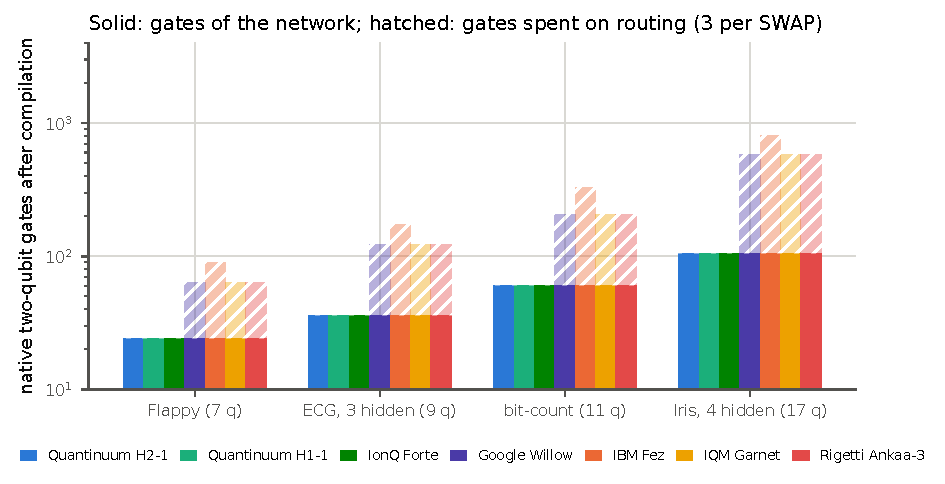
\includegraphics[width=\textwidth]{fig_hardware_entanglers}
\caption{Native two-qubit gates after compiling each network for each machine (our router;
log scale).  The all-to-all machines need only the network's own gates; the lattices spend most
of their budget on routing.  Run \run{hardware-plan/20260821T073211Z}.}
\label{fig:entanglers}
\end{figure}

\subsection{Expected fidelity}
\label{sec:fidelity}

\Cref{fig:fidelity} stacks the four factors of \cref{eq:fidelity} for the two smallest
circuits, with the exactly simulated total-variation distance between the compiled circuit run
clean and run under the machine's noise model next to each bar.  Flappy at 7 qubits is a
high-fidelity circuit on the trapped-ion machines ($F\approx 0.92$ on H2-1, $0.81$ on Forte),
marginal on Willow and Fez ($0.6$, $0.4$ with our router, $0.72$ with IBM's compiler), and poor on
Garnet ($0.18$).  Bit-count at 11 qubits is feasible on H-series ($0.81$) and Forte ($0.61$),
usable with IBM's compiler on Fez ($0.43$), and dead on Garnet ($0.004$), whose routed circuit
lasts $86\,\%$ of its $T_2$.  Two cautions.  The simulated distances of the \emph{compiled}
circuits ($0.03$ on H-series, $0.16$ on Forte, $0.43$ on Fez) are $5$--$15\times$ larger than
those of the uncompiled circuits in \cref{sec:noise-bitcount}: two native gates per controlled
rotation, resynthesised one-qubit gates and routing all cost.  And the vendors' two-qubit errors
are measured in isolation; IBM's own layered benchmark for Fez is $1.7\times$ worse than its
isolated gate error, so the lattice numbers are optimistic.

\begin{figure}[t]
\centering
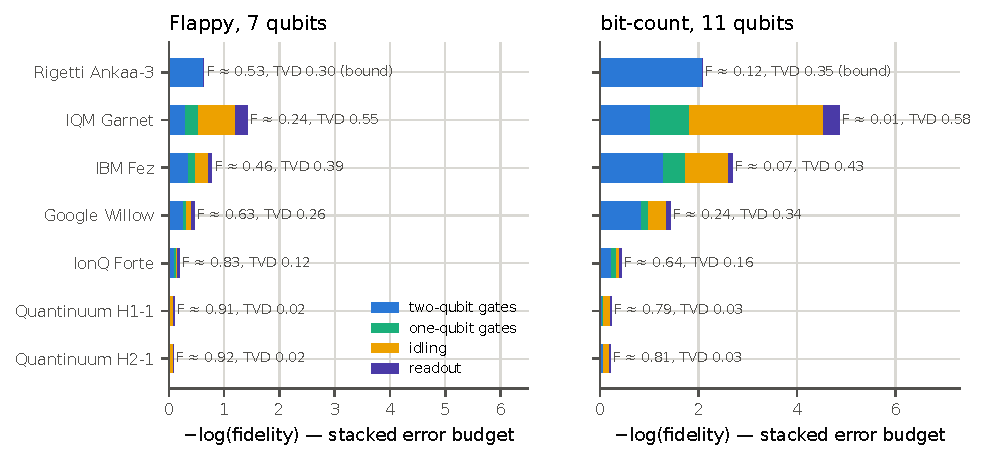
\includegraphics[width=\textwidth]{fig_hardware_fidelity}
\caption{Error budget per machine for the Flappy (left) and bit-count (right) circuits: the
stacked bars are $-\log$ of each factor of \cref{eq:fidelity}, so their total is $-\log F$;
the labels give $F$ and the simulated total-variation distance of the compiled circuit.
Quantinuum's idle term comes from its published memory error; Rigetti's is a bound (two-qubit
error only).}
\label{fig:fidelity}
\end{figure}

\subsection{Shots, time and money}
\label{sec:cost}

The shot budgets follow from \cref{sec:notation}.  An activation to $\pm 0.005$ needs
$10\,000$ shots.  The 32-bin bit-count histogram is estimated from the shots in which the
output fired ($\Pout = 0.487$ of them), and the plug-in KL is then biased upward by
$(K-1)/(2\cdot 0.487\cdot N) = 31.8/N$; reaching the trained model's $5.5\times10^{-4}$ needs
$58\,000$ shots, which we round to a $64\,000$-shot job.  The ECG denoiser's PSNR is capped by
shot noise at $10\log_{10}(4N)$: $2\,500$ shots per sample cap it at exactly $40$~dB, the
paper's Table~I value, and a $1\,800$-sample trace at $25\,000$ shots is $4.5\times10^7$ shots
--- ECG is a simulator experiment.  \Cref{fig:qpu-time} converts the circuit times to machine
time per job: milliseconds to two seconds on the superconducting machines, where the per-job
overhead dominates, but $72$\,s (Flappy) and $32$\,min (bit-count) on IonQ Forte, where the
circuit time does.  Prices (retrieved 20 August 2026; \cref{tab:cost}): a $4\,000$-shot Flappy
job costs about \$320 on Forte through Braket, \$6 on Garnet, $323$ Quantinuum credits
($\approx$\,\$4\,000 at the Azure plan rate), and is free on IBM's Open plan.  Training on
hardware is out of the question --- the paper's $2\,160$ evaluations at $64\,000$ shots are
$1.4\times10^8$ shots, $48$ days of Forte time or \$11\,M --- but fine-tuning the six output
angles ($90$ evaluations at $4\,000$ shots) is $1.8$ hours on Forte and about $45$ minutes on Fez.
Live Flappy play is equally out ($1\,500$ frames $\times$ $4\,000$ shots $\times$ $17.9$\,ms
$=30$ hours per episode on Forte); the falsifiable hardware observable is the activation map of
\cref{fig:flappy-policy} on a grid of observations, $16$ jobs.

\begin{table}[t]
\centering\small
\caption{Cost per job (numbers.md §cost).  IBM: \$1.60 per QPU second plus a 30\,s per-job
overhead (both assumptions, \cref{app:assumptions}); Quantinuum: the vendor's published credit
formula, converted at the Azure plan rate; Braket: published per-shot prices.}
\label{tab:cost}
\begin{tabularx}{\textwidth}{@{}l X l l@{}}
\toprule
Machine & model & Flappy, 4\,000 shots & bit-count, 64\,000 shots \\
\midrule
IBM Fez & \$1.60/s; 52\,ms resp.\ 1.8\,s of QPU & \$0.08 (\$48 with overhead) & \$2.85 (\$51) \\
IBM Open plan & 10 min per 28 days, free & \$0 & \$0 \\
Quantinuum H1/H2 & credits $=5 + (N_1 + 10N_2 + 5N_m)C/5000$ & 323 credits $\approx$ \$4\,030 & 11\,920 credits $\approx$ \$149\,000 \\
IonQ Forte (Braket) & \$0.30 + \$0.08/shot & \$320 & \$5\,120 \\
IQM Garnet (Braket) & \$0.30 + \$0.00145/shot & \$6.10 & \$93 \\
\bottomrule
\end{tabularx}
\end{table}

\begin{figure}[t]
\centering
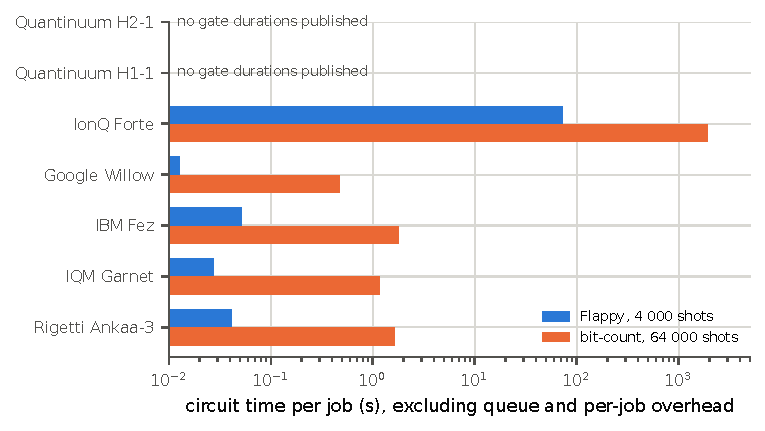
\includegraphics[width=0.75\textwidth]{fig_hardware_qpu_time}
\caption{Machine time per job, from the compiled circuit's duration (our router; readout
included where published).  Quantinuum publishes no durations.}
\label{fig:qpu-time}
\end{figure}

\subsection{Recommendation}
\label{sec:recommendation}

Run the 7-qubit Flappy activation map first: on IBM's free plan to debug the pipeline (readout
calibration, then zero-noise extrapolation by gate folding, both validated offline against the
noise model first), then on IonQ Forte for the confirmation (\$1\,300 for a $4\times4$ grid at
$1\,000$ shots), and on Quantinuum H2-1 for the headline number if an allocation exists.  The
bit-count histogram is feasible on H-series and Forte as a \emph{shape} demonstration but not as
a KL comparison (device error puts the KL floor at $10^{-2}$--$10^{-1}$, two orders above the
simulated $5.5\times10^{-4}$).  Iris is out of reach: loading the dataset state needs thousands
of two-qubit gates ($8\,166$ dense, $\approx 1\,440$ exploiting sparsity \cite{sbm,plesch,gleinig}),
giving a best-case fidelity near $0.2$ before the network runs.  Four things the code still
lacks for a live submission are listed in the repository's hardware plan (credentials, the
vendors' own routing, asynchronous job handles, readout-unfolding and folding utilities).
